\documentclass[openany]{tietreport}

\usepackage[utf8]{inputenc}
\usepackage[T1]{fontenc}
\usepackage{booktabs}
\usepackage{tabularx}
\usepackage{array}
\usepackage{enumitem}
\usepackage{tikz}
\usetikzlibrary{positioning,arrows.meta,shapes.geometric,fit,calc}
\usepackage{pgfplots}
\pgfplotsset{compat=1.16}
\usepackage[font=small,labelfont=bf]{caption}
\setlist{itemsep=1pt,topsep=3pt,parsep=0pt}
\hypersetup{colorlinks=true,linkcolor=black,citecolor=black,urlcolor=blue}
\renewcommand{\arraystretch}{1.12}

\usepackage[
  date=year,
  style=alphabetic,
  backend=biber,
  sorting=nty,
  maxnames=5,
  minnames=3,
  maxalphanames=4,
  minalphanames=3,
  doi=false,
  isbn=false,
  url=true,
  eprint=false
]{biblatex}
\addbibresource{references.bib}

%% ---------------- Title page ----------------
\TitlePageHeader{UCS503P -- Software Engineering Project Report}
\ProjectTitle{SkillBridge AI}
\ProjectSubTitle{An Intelligent Career Development and Placement-Readiness Platform for University Students}
\author{%
  \texttt{1024030168} Uday Dhir \\
  \texttt{1024030170} Aishwarya Verma%
}
\TitlePageSubText{Group: \texttt{CSE-04} BE Third Year, CSE}
\AdvisorName{Ms. Paramveer Kaur}
\TitlePageFooterText{{%
    \large End-Semester Evaluation \\[0.2cm]
    \bfseries Computer Science and Engineering Department}
  \\[0.15cm]
  Thapar Institute of Engineering and Technology, Patiala}

\newcommand{\code}[1]{\texttt{\small #1}}

\begin{document}
\maketitle
\tableofcontents

\chapter*{Abstract}
\addcontentsline{toc}{chapter}{Abstract}
Students preparing for campus placements use disconnected tools for resume review, coding practice and interview practice, and have no single, objective view of how ready they are. \textbf{SkillBridge AI} is a web platform that brings these activities together. A student uploads a PDF resume and receives an explainable 100-point ATS score with the detected skills; compares their skills against one of eleven role benchmarks to obtain a skill-gap report and a prioritised learning roadmap; solves coding problems that are auto-judged against hidden test cases; practises a text-based mock interview; and receives a single weighted \emph{Placement Readiness Score}. Recruiters can post jobs, search candidates and keep shortlists, and administrators can manage users and inspect an audit log.

The system is a modular monolith: a FastAPI/SQLAlchemy backend exposing 62 REST endpoints, a Next.js 14 frontend with thirteen pages, and a relational schema of sixteen tables. Where scoring is involved we deliberately chose documented, deterministic formulas over opaque models so that every score can be explained to the student.

This report documents the requirements, design, implementation and evaluation of the system, and reports measured results: the 32-test automated suite passes with 91\% line coverage once a resume-parser fallback defect found during final verification is fixed; resume upload-to-score takes a median of 24\,ms in-process; and on a 20-query retrieval benchmark, keyword (BM25) retrieval clearly outperforms the current hash-based ``dense'' component. Chapter~6 gives a candid review of limitations---most importantly an unsandboxed code-execution path and several security hardening gaps---together with remediation steps. The source code is available at \cite{repo}.

%% =====================================================================
\chapter{Introduction}

\section{Background and Context}
Campus recruitment compresses resume screening, online coding tests, technical interviews and behavioural rounds into a few weeks. Engineering students typically have a sound theoretical base but little visibility into what recruiters' automated screening and interview panels actually look for. Preparation is therefore scattered across resume-review conversations with seniors, coding-practice websites and informal mock interviews, none of which share data or give a combined picture of readiness.

SkillBridge AI addresses this by putting resume analysis, skill-gap detection, roadmap generation, coding assessment, mock interviews, job matching and analytics behind one authenticated web application, with separate portals for students, recruiters and administrators.

\subsection{Problem Statement}
Final-year and pre-final-year students face four recurring problems:
\begin{enumerate}
  \item \textbf{Fragmentation.} Resume feedback, coding practice and interview practice live in separate tools with no shared profile.
  \item \textbf{No objective benchmark.} Students cannot tell how their resume or skill set compares with what a role requires.
  \item \textbf{Slow, generic feedback.} Feedback is usually qualitative and arrives after the opportunity has passed.
  \item \textbf{Recruiter-side effort.} Recruiters and placement cells screen large candidate pools manually, with little tooling to filter and rank.
\end{enumerate}

\section{Project Objectives}
The objectives were stated in SMART form at the start of the project; the last column of Table~\ref{tab:objectives} records the outcome verified in Chapter~5.

\begin{table}[h]
\centering\small
\begin{tabularx}{\textwidth}{@{}l>{\raggedright\arraybackslash}X>{\raggedright\arraybackslash}p{1.45in}@{}}
\toprule
\textbf{ID} & \textbf{Objective} & \textbf{Outcome} \\
\midrule
O1 & Parse PDF resumes, extract skills against a five-category taxonomy and compute an explainable 100-point ATS score in under 5\,s & Met (median 24\,ms; PDF only) \\
O2 & Compare a student's skills with role benchmarks and generate a prioritised roadmap & Met (11 roles) \\
O3 & Provide auto-judged coding problems and a rubric-based mock interview & Met, with limitations (\S\ref{sec:limits}) \\
O4 & Combine four components into one transparent readiness score (35/20/25/20) & Met; one component is a placeholder \\
O5 & Apply sound engineering practice: layered architecture, RBAC, security headers, $>$80\% coverage & Partly met (91\% coverage; security gaps in \S\ref{sec:limits}) \\
\bottomrule
\end{tabularx}
\caption{Project objectives and outcomes.}
\label{tab:objectives}
\end{table}

\section{Scope}
\textbf{In scope:} student, recruiter, administrator and evaluator roles; PDF resume ingestion; skill taxonomy and benchmarks; roadmaps; Python coding assessment; text-based mock interviews; job matching; analytics dashboard; containerised deployment and CI.

\textbf{Out of scope for this semester:} voice or video interviews, multi-language code execution, live external job-market data, DOCX parsing, and calendar integration. These are listed as future work in Chapter~7.

\section{Organisation of the Report}
Chapter~2 reviews related techniques. Chapter~3 presents requirements and design, Chapter~4 the implementation, and Chapter~5 the testing and measured results. Chapter~6 critically reviews limitations and security findings, and Chapter~7 concludes with future work.

%% =====================================================================
\chapter{Related Work and Background}

\paragraph{Applicant tracking and resume scoring.} Commercial ATS products parse a resume into sections and keywords and rank candidates against a job description. Their scoring is proprietary, which leaves students guessing. We therefore implement a transparent rubric (Section~\ref{sec:ats}) whose four components are shown to the user.

\paragraph{Hybrid retrieval.} Retrieval-Augmented Generation (RAG) \cite{lewis2020rag} grounds generated content in retrieved documents. Sparse keyword scoring such as BM25 \cite{robertson2009bm25} matches exact technical terms, whereas dense embeddings capture paraphrase. Reciprocal Rank Fusion (RRF) \cite{cormack2009rrf} merges the two ranked lists without needing comparable score scales:
\begin{equation}
  \mathrm{RRF}(d) = \sum_{r \in \{\text{dense},\,\text{sparse}\}} \frac{1}{k + \mathrm{rank}_r(d)}, \qquad k = 60.
\end{equation}
Sentence-BERT style encoders \cite{reimers2019sbert} are the usual source of dense vectors.

\paragraph{Web security.} The OWASP Top~10 \cite{owasp} guided the choice of security headers, role-based access control and input validation, and JSON Web Tokens \cite{rfc7519} are used for stateless authentication.

\paragraph{Software engineering practice.} The project follows a requirements $\rightarrow$ design $\rightarrow$ implementation $\rightarrow$ test lifecycle \cite{sommerville2016,pressman2020}, delivered in milestones M0--M11 (foundation, authentication, resumes, skill gap, RAG and roadmaps, assessments, interviews, jobs, analytics, recruiter/admin, security, verification).

%% =====================================================================
\chapter{Requirements and System Design}

\section{Actors and Functional Requirements}
Four roles are enforced by role-based access control: \code{STUDENT}, \code{RECRUITER}, \code{ADMIN} and \code{EVALUATOR}. Table~\ref{tab:fr} lists the principal functional requirements.

\begin{table}[h]
\centering\small
\begin{tabularx}{\textwidth}{@{}l>{\raggedright\arraybackslash}p{0.95in}>{\raggedright\arraybackslash}X@{}}
\toprule
\textbf{ID} & \textbf{Actor} & \textbf{Requirement} \\
\midrule
FR1 & All & Register, log in, refresh an access token, view own profile \\
FR2 & Student & Upload a PDF resume and view parsed skills, ATS score and weak sections \\
FR3 & Student & Run a skill-gap analysis against a target role benchmark \\
FR4 & Student & Generate a roadmap and mark roadmap items complete \\
FR5 & Student & Attempt coding questions and view per-test results \\
FR6 & Student & Take a mock-interview session and receive per-answer and summary feedback \\
FR7 & Student & View job recommendations with an explainable match breakdown \\
FR8 & Student & View a composite readiness dashboard with a suggested next action \\
FR9 & Recruiter & Create, edit and delete job postings; search candidates; manage a shortlist \\
FR10 & Admin & View platform statistics, manage user activation, inspect the audit log \\
FR11 & All & Search the curriculum index through hybrid retrieval \\
\bottomrule
\end{tabularx}
\caption{Principal functional requirements.}
\label{tab:fr}
\end{table}

Non-functional targets were: resume feedback in under 5\,s, API latency under 100\,ms for non-blocking endpoints, test coverage above 80\%, and a reproducible containerised deployment.

\section{Architecture}
SkillBridge AI is a \emph{modular monolith}: one deployable backend with strict internal layering, chosen over microservices to keep transactions simple and testing cheap for a two-person, single-semester project. Figure~\ref{fig:arch} shows the three tiers.

\begin{figure}[h]
\centering
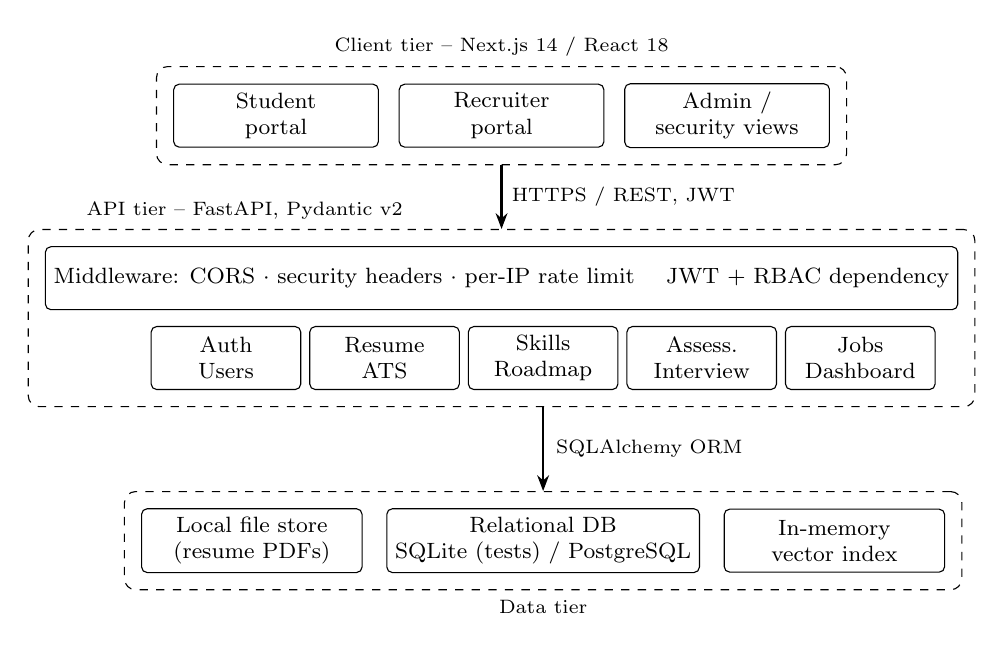
\begin{tikzpicture}[
  box/.style={draw,rounded corners=2pt,align=center,font=\footnotesize,minimum height=0.8cm,inner sep=3pt},
  tier/.style={draw,dashed,rounded corners=4pt,inner sep=6pt},
  arr/.style={-{Stealth[length=2mm]},thick}]
  \node[box,minimum width=2.6cm] (stu) {Student\\portal};
  \node[box,minimum width=2.6cm,right=0.25cm of stu] (rec) {Recruiter\\portal};
  \node[box,minimum width=2.6cm,right=0.25cm of rec] (adm) {Admin /\\security views};
  \node[tier,fit=(stu)(rec)(adm),label={[font=\scriptsize]above:Client tier -- Next.js 14 / React 18}] (c) {};

  \node[box,minimum width=8.9cm,below=1.25cm of rec] (mw) {Middleware: CORS $\cdot$ security headers $\cdot$ per-IP rate limit \quad JWT + RBAC dependency};
  \node[box,below=0.2cm of mw,xshift=-3.5cm,minimum width=1.9cm] (s1) {Auth\\Users};
  \node[box,right=0.1cm of s1,minimum width=1.9cm] (s2) {Resume\\ATS};
  \node[box,right=0.1cm of s2,minimum width=1.9cm] (s3) {Skills\\Roadmap};
  \node[box,right=0.1cm of s3,minimum width=1.9cm] (s4) {Assess.\\Interview};
  \node[box,right=0.1cm of s4,minimum width=1.9cm] (s5) {Jobs\\Dashboard};
  \node[tier,fit=(mw)(s1)(s5),label={[font=\scriptsize]above left:API tier -- FastAPI, Pydantic v2}] (a) {};

  \node[box,below=1.5cm of s3,minimum width=3.4cm] (db) {Relational DB\\SQLite (tests) / PostgreSQL};
  \node[box,left=0.3cm of db,minimum width=2.8cm] (fs) {Local file store\\(resume PDFs)};
  \node[box,right=0.3cm of db,minimum width=2.8cm] (vs) {In-memory\\vector index};
  \node[tier,fit=(fs)(db)(vs),label={[font=\scriptsize]below:Data tier}] (d) {};

  \draw[arr] (c.south) -- node[right,font=\scriptsize]{HTTPS / REST, JWT} (a.north -| c.south);
  \draw[arr] (a.south -| db.north) -- node[right,font=\scriptsize,xshift=1pt]{SQLAlchemy ORM} (d.north -| db.north);
\end{tikzpicture}
\caption{Three-tier architecture of SkillBridge AI as implemented.}
\label{fig:arch}
\end{figure}

The backend is organised into four layers per feature: \code{api/v1} (routers), \code{services} (business logic), \code{schemas} (Pydantic request/response models) and \code{models} (SQLAlchemy entities). Routers never contain scoring logic, which makes each formula unit-testable in isolation.

\section{Technology Stack}
\begin{table}[h]
\centering\small
\begin{tabularx}{\textwidth}{@{}l>{\raggedright\arraybackslash}X@{}}
\toprule
\textbf{Concern} & \textbf{Technology} \\
\midrule
Backend & Python, FastAPI \cite{fastapi}, Uvicorn, Pydantic v2 \\
Persistence & SQLAlchemy 2 \cite{sqlalchemy}; SQLite for tests, PostgreSQL 16 in Docker Compose \\
Frontend & Next.js 14 (App Router) \cite{nextjs}, React 18, TypeScript \\
PDF extraction & \code{pdfplumber}, with \code{pypdf} and raw-byte fallbacks \\
Security & PyJWT (HS256), \code{bcrypt}, custom Starlette middleware \\
Testing & Pytest, \code{pytest-cov}, FastAPI \code{TestClient} \\
DevOps & Dockerfiles for both tiers, Docker Compose, GitHub Actions \\
\bottomrule
\end{tabularx}
\caption{Technologies actually used by the application code.}
\label{tab:stack}
\end{table}

\noindent Docker Compose also provisions Qdrant, Redis and MinIO containers, and the dependency list includes \code{qdrant-client} and \code{redis}. The application code does not yet call them: the vector index is an in-process list, resumes are stored on local disk, and rate-limit state is in memory. They are provisioned as the intended production back-ends (see Chapter~7).

\section{Data Model}
The schema has sixteen tables (Table~\ref{tab:db}); it is created with \code{Base.metadata.create\_all} at start-up.

\begin{table}[h]
\centering\small
\begin{tabularx}{\textwidth}{@{}l>{\raggedright\arraybackslash}X@{}}
\toprule
\textbf{Group} & \textbf{Tables} \\
\midrule
Identity & \code{users}, \code{student\_profiles}, \code{recruiter\_profiles}, \code{refresh\_tokens}, \code{audit\_logs} \\
Resume \& skills & \code{resume\_documents}, \code{role\_benchmarks}, \code{skill\_gap\_analyses} \\
Roadmap & \code{career\_roadmaps}, \code{roadmap\_items} \\
Assessment & \code{assessment\_questions}, \code{assessment\_submissions} \\
Interview & \code{interview\_sessions}, \code{interview\_exchanges} \\
Jobs \& recruiting & \code{job\_postings}, \code{recruiter\_shortlists} \\
\bottomrule
\end{tabularx}
\caption{Database tables grouped by feature.}
\label{tab:db}
\end{table}

\section{API Surface}
The backend exposes 62 endpoints under \code{/api/v1}, summarised in Table~\ref{tab:api}. All routes other than registration, login, refresh and health require a bearer token, and role checks are applied through a reusable \code{RoleChecker} dependency.

\begin{table}[h]
\centering\small
\begin{tabular}{@{}lc@{\hspace{2em}}lc@{\hspace{2em}}lc@{}}
\toprule
\textbf{Module} & \textbf{\#} & \textbf{Module} & \textbf{\#} & \textbf{Module} & \textbf{\#} \\
\midrule
auth & 4 & roadmaps & 4 & recruiter & 5 \\
users & 2 & assessments & 6 & admin & 6 \\
resumes & 6 & interviews & 9 & dashboard & 5 \\
skills & 5 & jobs & 7 & rag / health & 2 / 1 \\
\bottomrule
\end{tabular}
\caption{Endpoint count per router module (total 62).}
\label{tab:api}
\end{table}

\section{Security Design}
The following controls are implemented in code and covered by tests unless stated otherwise.
\begin{itemize}
  \item \textbf{Passwords:} bcrypt with a per-password salt (input truncated to bcrypt's 72-byte limit).
  \item \textbf{Tokens:} HS256 JWTs. Access tokens expire after 15 minutes and carry the role and a unique \code{jti}; refresh tokens last 7 days and are stored in the database.
  \item \textbf{RBAC:} a dependency rejects a token whose role is not allowed for the route with HTTP 403.
  \item \textbf{Headers:} \code{X-Frame-Options: DENY}, \code{X-Content-Type-Options: nosniff}, \code{Strict-Transport-Security}, \code{Content-Security-Policy} and \code{X-XSS-Protection} on every response.
  \item \textbf{Rate limiting:} a fixed-window, in-memory per-IP limiter returning HTTP 429 above 1000 requests per minute.
  \item \textbf{Input validation:} Pydantic schemas on every request body; PDF uploads must have a \code{.pdf} name, the \code{\%PDF-} magic bytes and be at most 10\,MB.
  \item \textbf{Auditability:} registration, login, resume upload and analyses write rows to \code{audit\_logs}, which administrators can view.
\end{itemize}
Gaps against this baseline are reported in Chapter~6.

%% =====================================================================
\chapter{Implementation}

\section{Resume Intelligence and ATS Scoring}
\label{sec:ats}
On upload the file is validated, saved, and its text extracted with \code{pdfplumber}. If that fails or returns no text, extraction falls back to \code{pypdf} and finally to a raw byte decode, so a malformed file degrades gracefully rather than failing the request. The text is lower-cased and matched with word-boundary regular expressions against a taxonomy of five categories: programming languages (15 terms), frameworks and libraries (17), databases and vector stores (10), DevOps and cloud (12), and AI/ML/RAG (9). The extractor also finds an e-mail address, detects which of five standard sections are present (education, projects, experience, skills, certifications), and flags weak bullet lines that contain neither an action verb nor a quantified metric.

The ATS score is an inspectable sum of four components, clamped to $[50,98]$:
\begin{align}
S_{\mathrm{sec}} &= \min(30,\, 6\,N_{\mathrm{sections}}), &
S_{\mathrm{skill}} &= \min(40,\, 5\,N_{\mathrm{skills}}),\\
S_{\mathrm{contact}} &= 10\,[\text{email}] + 5\,[\text{length}>200], &
S_{\mathrm{bullet}} &= 10\,[\text{action verb}] + 5\,[\text{metric}],
\end{align}
\begin{equation}
  \mathrm{ATS} = \min\bigl(98,\ \max(50,\ S_{\mathrm{sec}}+S_{\mathrm{skill}}+S_{\mathrm{contact}}+S_{\mathrm{bullet}})\bigr).
\end{equation}
All four component values are returned to the client, so a student can see exactly where points were lost. The resume is also compared with a pasted job description by taking the overlap of detected skills (bounded to 40--100\%), and newly detected skills are merged into the student's profile.

\section{Skill-Gap Analysis and Roadmaps}
Eleven role benchmarks (e.g.\ Frontend Developer, Backend Engineer, Data Scientist, DevOps Engineer, AI/ML RAG Specialist) each list required and optional skills. With $R_{\mathrm{req}}$ and $R_{\mathrm{opt}}$ the fractions of required and optional skills the student already has,
\begin{equation}
  S_{\mathrm{gap}} = 100\,(0.85\,R_{\mathrm{req}} + 0.15\,R_{\mathrm{opt}}).
\end{equation}
Role lookup tolerates spelling variants (``Full Stack'' vs.\ ``Fullstack''). A roadmap is built by listing missing required skills first, then missing optional ones, and querying the hybrid curriculum index with ``\emph{role skill}'' to attach the best-matching learning module to each item, together with an hour estimate. Items can be marked completed and completion rate feeds the dashboard.

\section{Hybrid Curriculum Retrieval}
The curriculum index holds learning-module records (title, skill, category, content). A query is ranked twice: by cosine similarity between 1536-dimensional unit vectors (dense), and by a simple term-overlap score normalised by document length (sparse). The two rankings are merged with RRF, $k=60$ (Eq.~2.1). Embeddings are obtained from the OpenAI embeddings endpoint when an API key is configured; otherwise a deterministic SHA-256-derived vector is used so that the system works offline and tests are repeatable. The consequences of this fallback are quantified in Section~\ref{sec:rag}.

\section{Coding Assessment}
Three seeded Python problems (easy, medium, hard) each carry hidden test cases. A submission must define \code{solution(...)}; the engine executes it, calls it on each test input, compares with the expected value and records pass/fail, exception messages, wall-clock time and a score equal to the percentage of tests passed. The current executor runs submitted code in-process (see Section~\ref{sec:limits}).

\section{Mock Interview}
A session draws three questions for the chosen role (Backend Engineer, Fullstack Developer, AI/ML RAG Specialist, or a default set), covering technical architecture, system design and a behavioural STAR question. Each typed answer receives a score from a transparent rubric: answers under 15 words score 40; otherwise
\begin{equation}
  S_{\mathrm{ans}} = \min\bigl(100,\ 65 + \min(20,\ 0.2\,W) + \min(15,\ 3K)\bigr),
\end{equation}
where $W$ is the word count and $K$ the number of distinct technical keywords from a fixed list. Behavioural answers are additionally checked for situation and result cues, and feedback text lists improvements. The session score is the mean of answer scores, mapped to a three-band summary.

\section{Job Matching, Readiness Score and Portals}
\paragraph{Job match.} Each posting lists required and optional skills; the match uses the same 85/15 weighting as the skill gap and returns matching skills, missing required skills and a one-sentence explanation.

\paragraph{Placement Readiness Score.} The dashboard combines four components:
\begin{equation}
  R = 0.35\,S_{\mathrm{gap}} + 0.20\,S_{\mathrm{resume}} + 0.25\,S_{\mathrm{coding}} + 0.20\,S_{\mathrm{interview}}.
\end{equation}
$S_{\mathrm{coding}}$ and $S_{\mathrm{interview}}$ are the means of the student's submissions and completed sessions. A rule-based ``next best action'' picks the first unmet step (upload resume, run gap analysis, continue roadmap, attempt assessments, practise interview, explore jobs). \emph{Note:} $S_{\mathrm{resume}}$ is currently a constant 75 once any resume exists rather than the stored ATS score; this is listed in Table~\ref{tab:findings}.

\paragraph{Recruiter and admin portals.} Recruiters manage postings, search students by skill, and keep shortlists. Administrators see platform statistics, activate or deactivate accounts, and read the audit log.

\section{Frontend}
The Next.js App Router frontend has thirteen routes: landing, login, register, dashboard, resumes, skills, roadmap, assessments, interviews, jobs, analytics, recruiter and admin, plus a security page. An \code{AuthContext} stores the tokens, and a small typed fetch wrapper (\code{lib/api.ts}) calls the backend with the bearer token and normalises validation errors for display. The UI uses a dark, glass-style design system with CSS variables, semantic HTML and ARIA labels.

\section{Build, Deployment and CI}
Each tier has a Dockerfile; \code{docker-compose.yml} starts PostgreSQL, Qdrant, Redis and MinIO; \code{start.bat}/\code{stop.bat} wrap local start-up on Windows. A GitHub Actions workflow runs the backend Pytest suite and a Next.js production build on every push to \code{main} or \code{develop} and on pull requests to \code{main}.

%% =====================================================================
\chapter{Testing and Results}

\section{Methodology}
Testing was automated at the API level. The suite has \textbf{32 tests} in twelve files, run with Pytest and FastAPI's \code{TestClient} against an SQLite database; most tests register users, authenticate, and exercise complete flows, so they act as integration tests that also cover the service-layer formulas. Table~\ref{tab:tests} lists tests per area. All figures in this chapter were measured by re-running the suite and scripts in a clean environment (Python~3.12, \code{pdfplumber}~0.11.10, FastAPI~0.165) rather than copied from earlier documents.

\begin{table}[h]
\centering\small
\begin{tabular}{@{}lc@{\hspace{2em}}lc@{\hspace{2em}}lc@{}}
\toprule
\textbf{Area} & \textbf{Tests} & \textbf{Area} & \textbf{Tests} & \textbf{Area} & \textbf{Tests} \\
\midrule
Authentication & 7 & Skills & 3 & Jobs & 2 \\
Resumes & 5 & Security & 4 & Recruiter/admin & 2 \\
Assessments & 2 & Health & 2 & RAG & 2 \\
Roadmaps & 1 & Dashboard & 1 & Interviews & 1 \\
\bottomrule
\end{tabular}
\caption{Automated tests per area (total 32).}
\label{tab:tests}
\end{table}

\section{Functional and Coverage Results}
\label{sec:cov}
On the committed code with current library versions, \textbf{28 of 32 tests pass and four resume tests fail}. The cause is a real defect: the text extractor fell back to \code{pypdf} only when \code{pdfplumber} was \emph{missing}; when \code{pdfplumber} raised on a malformed PDF the exception propagated. Broadening the handler as described in Section~4.1 (a 20-line change, supplied in Appendix~A) makes \textbf{all 32 tests pass}. The results below are for the fixed code.

\begin{table}[h]
\centering\small
\begin{tabular}{@{}lrrr@{}}
\toprule
\textbf{Module (selected)} & \textbf{Statements} & \textbf{Missed} & \textbf{Coverage} \\
\midrule
\code{services/resume\_parser} & 92 & 10 & 89\% \\
\code{services/vector\_store} & 55 & 6 & 89\% \\
\code{services/interview\_engine} & 45 & 6 & 87\% \\
\code{services/assessment\_engine} & 48 & 7 & 85\% \\
\code{services/dashboard} & 62 & 15 & 76\% \\
\code{core/security} & 34 & 2 & 94\% \\
\code{core/middleware} & 33 & 2 & 94\% \\
\code{api/v1/auth} & 65 & 13 & 80\% \\
\code{api/v1/users} & 29 & 12 & 59\% \\
\midrule
\textbf{Total (all of \code{app/})} & \textbf{1918} & \textbf{167} & \textbf{91\%} \\
\bottomrule
\end{tabular}
\caption{Line coverage with the parser fix applied (32 tests, about 25\,s).}
\label{tab:cov}
\end{table}

\section{Performance}
Table~\ref{tab:perf} reports in-process measurements (no network). They indicate algorithmic cost, not production latency, and the resume used was a one-page, text-based PDF.

\begin{table}[h]
\centering\small
\begin{tabular}{@{}lccc@{}}
\toprule
\textbf{Measurement} & \textbf{Target} & \textbf{Measured} & \textbf{Samples} \\
\midrule
Resume upload $\rightarrow$ ATS score (median) & $<5$\,s & 24\,ms & 30 \\
Resume upload $\rightarrow$ ATS score (p95) & $<5$\,s & 28\,ms & 30 \\
Authenticated \code{GET /auth/me} (median) & $<100$\,ms & 4.8\,ms & 100 \\
\code{GET /health} (median) & $<100$\,ms & 3.2\,ms & 200 \\
ATS determinism (same file, 30 uploads) & identical & 1 distinct score (98) & 30 \\
\bottomrule
\end{tabular}
\caption{Measured performance.}
\label{tab:perf}
\end{table}

\noindent The ATS rubric is deterministic by construction. For the test resume the breakdown was section 30/30, skills 40/40 (13 skills detected, capped), contact 15/15 and bullets 15/15.

\section{Retrieval Evaluation}
\label{sec:rag}
To check whether hybrid retrieval behaves as intended, we built a small benchmark (script in the repository's evaluation folder, Appendix~A): the five seeded curriculum modules and 20 queries with one known relevant module each, half \emph{keyword} queries that reuse terms from the document and half \emph{paraphrase} queries that do not (e.g.\ ``make slow SQL queries faster''). The offline hash-based embedding was used, i.e.\ with no API key. We report Precision@1 and Mean Reciprocal Rank (MRR); chance MRR for five documents is 0.457.

\begin{table}[h]
\centering\small
\begin{tabular}{@{}l ccc ccc@{}}
\toprule
 & \multicolumn{3}{c}{\textbf{All queries ($n=20$)}} & \multicolumn{3}{c}{\textbf{Paraphrase ($n=10$)}} \\
\cmidrule(lr){2-4}\cmidrule(lr){5-7}
\textbf{Method} & P@1 & Hit@3 & MRR & P@1 & Hit@3 & MRR \\
\midrule
Dense (hash embedding) & 0.15 & 0.65 & 0.432 & 0.10 & 0.80 & 0.433 \\
Sparse term overlap & 0.75 & 0.95 & 0.852 & 0.50 & 0.90 & 0.703 \\
RRF hybrid & 0.45 & 1.00 & 0.708 & 0.50 & 1.00 & 0.717 \\
\bottomrule
\end{tabular}
\caption{Retrieval results on the five-document curriculum index.}
\label{tab:rag}
\end{table}

\begin{figure}[h]
\centering
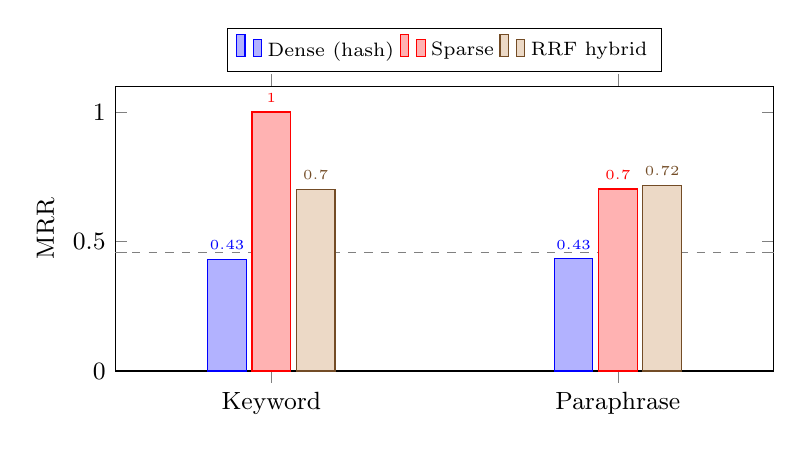
\begin{tikzpicture}
\begin{axis}[
  ybar, bar width=14pt, width=0.82\textwidth, height=5.2cm,
  ymin=0, ymax=1.1, ylabel={MRR}, ylabel style={font=\small},
  symbolic x coords={Keyword,Paraphrase}, xtick=data,
  enlarge x limits=0.45, legend style={font=\scriptsize,at={(0.5,1.05)},anchor=south,legend columns=-1},
  tick label style={font=\small}, nodes near coords, every node near coord/.append style={font=\tiny},
  extra y ticks=0.457, extra y tick labels={}, extra y tick style={grid=major,grid style={dashed,gray}}]
\addplot coordinates {(Keyword,0.432)(Paraphrase,0.433)};
\addplot coordinates {(Keyword,1.000)(Paraphrase,0.703)};
\addplot coordinates {(Keyword,0.700)(Paraphrase,0.717)};
\legend{Dense (hash), Sparse, RRF hybrid}
\end{axis}
\end{tikzpicture}
\caption{MRR by query type. The dashed line marks chance level (0.457).}
\label{fig:rag}
\end{figure}

\paragraph{Interpretation.} The hash-based dense component performs at chance level, which is expected: a hash of the text has no notion of meaning, so only identical strings are similar. Consequently fusing it with the sparse ranking \emph{lowers} MRR relative to sparse alone (0.708 vs.\ 0.852), although RRF does keep the relevant module in the top three for every query. The benchmark is small (five documents, 20 queries) and the sparse method benefits from queries built from the same domain vocabulary, so the absolute numbers should not be generalised. The result nevertheless shows that the hybrid design only pays off with real semantic embeddings; with the OpenAI path or a local Sentence-BERT model the dense arm would be expected to help on paraphrases, but we have not measured this.

\section{Summary of Results}
Against the objectives in Table~\ref{tab:objectives}: speed, determinism and test targets were met with wide margins; coverage exceeds the 80\% goal; retrieval quality with offline embeddings is below what the architecture promises; and the security items in the next chapter show that the hardening goal was only partly achieved.

%% =====================================================================
\chapter{Critical Review: Limitations and Findings}
\label{sec:limits}
A final verification pass compared the code against earlier project documents. This chapter records what we found. Several statements in the earlier audit documents (for example Argon2id hashing, RS256 signing, a 5-request/minute authentication limit and account lockout) do not match the code and are \emph{not} claimed in this report.

\begin{table}[h]
\centering\footnotesize
\begin{tabularx}{\textwidth}{@{}c>{\raggedright\arraybackslash}p{0.62in}>{\raggedright\arraybackslash}X>{\raggedright\arraybackslash}X@{}}
\toprule
\textbf{\#} & \textbf{Severity} & \textbf{Finding (verified)} & \textbf{Remediation} \\
\midrule
1 & High & Submitted code is run with in-process \code{exec}; a test submission successfully imported \code{os} and listed the server directory. No time limit, so an infinite loop blocks a worker. & Run in a subprocess or container with CPU, memory and time limits, no network, and restricted filesystem. \\
2 & High & Default JWT secret and database/object-store passwords are in source and Compose; CORS allow-list contains \code{"*"}. & Require secrets from the environment, fail on defaults, strict origins. \\
3 & Medium & Rate limit is global (1000/min/IP); no per-route limit on login, no account lockout, no logout endpoint, refresh tokens are not rotated or revoked. & Add a login limiter and lockout, rotate refresh tokens, add logout. \\
4 & Medium & \code{requirements.txt} lacks PyJWT, bcrypt and email-validator, so a clean install cannot import the app; CI would fail on a fresh runner. & Add the three packages and pin versions. \\
5 & Medium & Resume text extraction did not fall back on parser errors (four tests failed). & Fix supplied (Appendix~A). \\
6 & Medium & Offline embeddings are hash-based, so dense retrieval is at chance level (Table~\ref{tab:rag}). Qdrant, Redis and MinIO are provisioned but unused. & Use a Sentence-BERT model or API embeddings; connect Qdrant. \\
7 & Low & Interview scoring is a length and keyword heuristic and can be gamed by keyword stuffing. & Add an LLM-based rubric grader with schema validation. \\
8 & Low & Dashboard resume score is a constant 75 instead of the ATS score. & Read the stored ATS score. \\
9 & Low & Only PDF resumes are parsed; ATS score is clamped to 50--98, so a poor resume still shows 50. & Add DOCX; show the unclamped score. \\
10 & Low & The \code{/security} page lists static ``pass'' items that do not reflect the backend; the landing page mentions audio interviews that are not implemented. & Generate the page from real checks; correct the copy. \\
11 & Low & Schema is created with \code{create\_all} (no migrations); the frontend \code{test} script is a stub. & Add Alembic and component tests. \\
\bottomrule
\end{tabularx}
\caption{Verified limitations and recommended remediation.}
\label{tab:findings}
\end{table}

\paragraph{Why the first item matters most.} The assessment endpoint is available to any registered student; the engineering consequence is that a single malicious submission can read files, environment variables (including secrets) or exhaust the server. Until it is sandboxed the platform should not be exposed to untrusted users.

\paragraph{Challenges and how they were handled.} Resumes vary widely in layout, so extraction uses a layered fallback; stateful rate limiting without Redis was solved with an in-memory window, acceptable for a single process but not for multiple replicas; and keeping scores explainable meant favouring simple formulas over learned models, at the cost of sophistication.

%% =====================================================================
\chapter{Conclusion and Future Work}

\section{Summary of Work}
We designed and built a working multi-role career-readiness platform: a layered FastAPI backend with 62 endpoints and sixteen tables, a thirteen-route Next.js frontend, explainable scoring for resumes, skill gaps, interviews, jobs and overall readiness, a hybrid retrieval component, containerised deployment and a CI workflow. The automated suite of 32 tests passes with 91\% coverage after the parser fix, and core scoring runs in tens of milliseconds.

\section{Key Learnings}
\begin{enumerate}
  \item \textbf{Explainability helps users.} Showing the four ATS components makes feedback actionable and the score reproducible.
  \item \textbf{Verify claims against the code.} Writing documents and dashboards ahead of the implementation produced statements that were not true; measuring, as in Chapter~5, is the only reliable record.
  \item \textbf{Hybrid retrieval depends on its parts.} Fusion cannot rescue a dense component with no semantic signal.
  \item \textbf{A modular monolith suited the scale}, giving simple transactions and fast, cheap tests.
\end{enumerate}

\section{Future Work}
\begin{enumerate}
  \item Sandbox code execution in containers with resource limits, then add more languages.
  \item Harden authentication: login rate limits, lockout, refresh rotation, logout, RS256 or managed secrets, Argon2id.
  \item Replace hash embeddings with real embeddings, move the index to Qdrant, and evaluate on a larger labelled set.
  \item LLM-based interview grading with structured output and a deterministic fallback; optionally voice input.
  \item DOCX support, S3-compatible resume storage, Alembic migrations and Redis-backed rate limiting.
  \item Measure effectiveness with real students, for instance by relating readiness scores to placement outcomes.
\end{enumerate}

\printbibliography[heading=bibintoc,title={Bibliography}]

\appendix
\chapter{Reproducing the Results}
\textbf{Tests and coverage:} from \code{backend/}, install dependencies (adding \code{PyJWT}, \code{bcrypt}, \code{email-validator}), then run \code{pytest -q --cov=app}. \textbf{Parser fix:} apply \code{resume\_parser\_fix.patch}, which replaces \code{extract\_text\_from\_pdf} with the layered \code{pdfplumber}~$\rightarrow$~\code{pypdf}~$\rightarrow$~raw-byte version described in Section~4.1. \textbf{Performance and retrieval:} run \code{eval/measure.py} from \code{backend/}; it uploads a generated PDF 30 times, times three endpoints, and computes P@1, Hit@3 and MRR for the dense, sparse and RRF rankers on the 20 queries of Section~5.3.

\end{document}
